\documentclass[12pt]{article}
\usepackage[top=1in,bottom=1in,left=0.75in,right=1in]{geometry}
\usepackage{alltt}
\usepackage{array}	
\usepackage{graphicx}
\usepackage{tabularx}
\usepackage{verbatim}
\usepackage{setspace}
\usepackage{listings}
\usepackage{amssymb,amsmath, amsthm}
\usepackage{qtree}
\usepackage{oz}
\usepackage[cc]{titlepic}
\usepackage{fancyvrb}

\title{Concordia University\\
Department of Computer Science and Software Engineering\\
\textbf{SOEN 331 - S and U\\Introduction to Formal Methods\\for Software Engineering}\\
\ \\
\textbf{Assignment 2 - Solutions}\\
The Object-Z specification language\\
\textbf{Team 19 - Section U}}
\author{
	\textbf{Samuel Boaknin}\\
	\texttt{40009692}
	\and
	\textbf{Ryan Leyland}\\
	\texttt{40015165}
	\and
	\textbf{Saleha Tariq}\\
	\texttt{40006997}
	\and
	\textbf{Meng Susana Ung}\\
	\texttt{40099729}
}
\date{Due Date: March 11, 2021}

\begin{document}
\begin{spacing}{1.5}

\maketitle

\newpage

\section{Contact management}
\subsection{State}
%State content
\begin{enumerate}
\item This is our diagram for the state of the system:\\
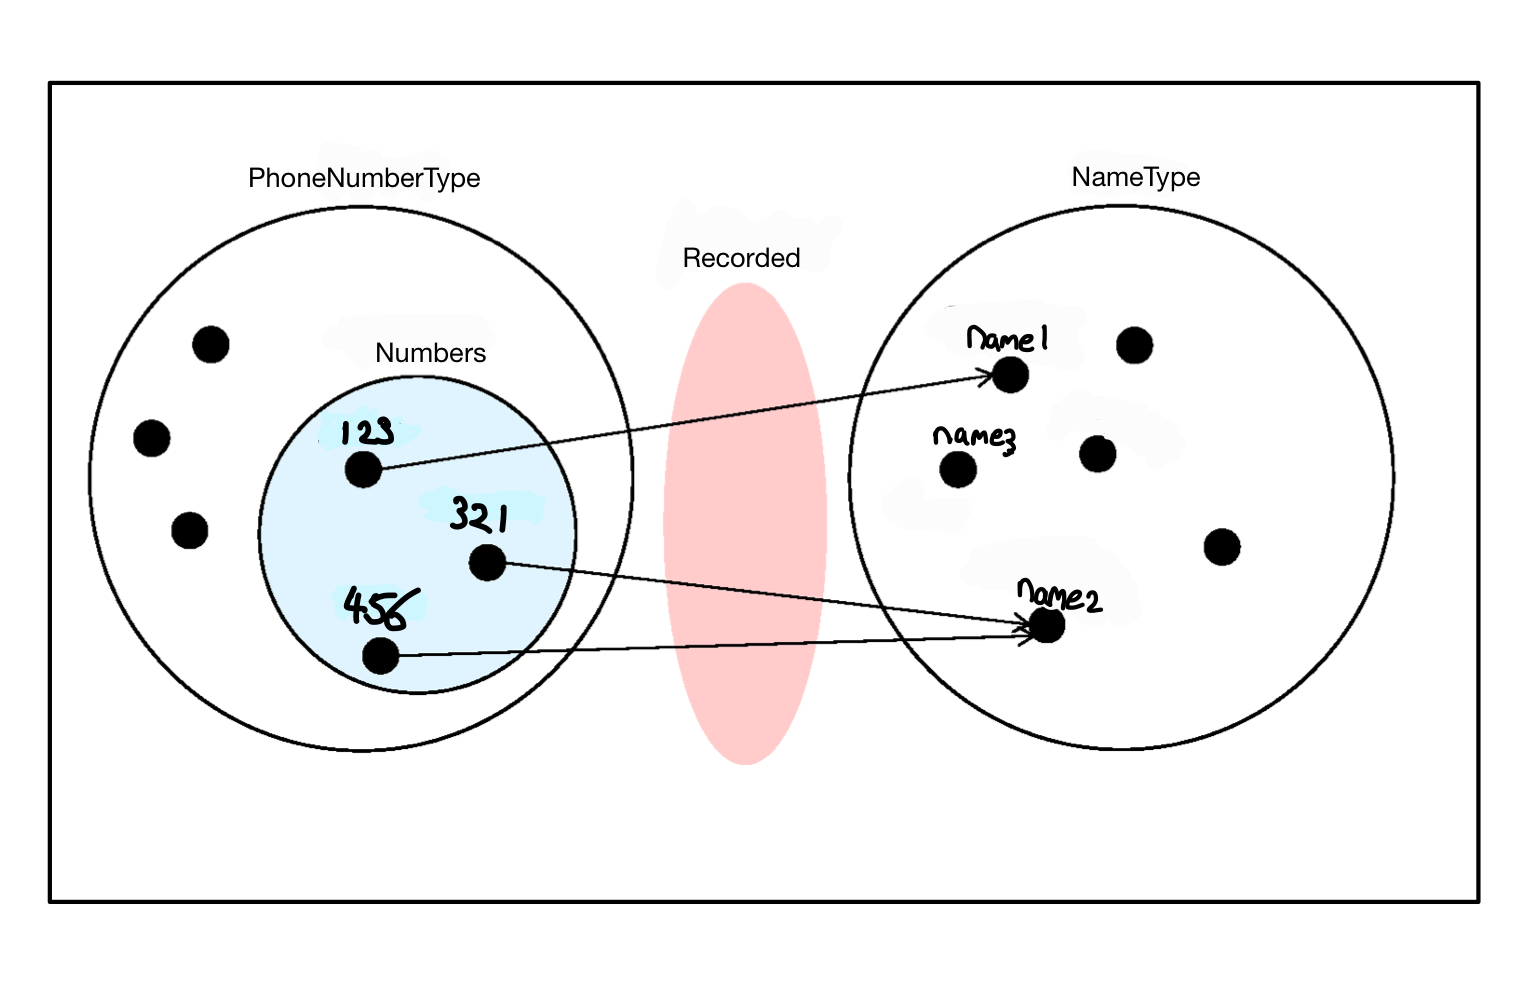
\includegraphics[scale=.25]{state-diagram}
\item The formal definition of \emph{numbers} is as follows:
\[ numbers \ : \ \mathbb{P}\ PhoneNumberType \]
\item The relation \emph{recorded} must indeed be captured by a function. A function, by definition, enforces that each element of a source set (that is, the set in the domain) is mapped to exactly one element of a target set (a set of elements in the range). Part of the requirements for the system is that people may not share phone numbers. By making \emph{recorded} a function, and setting the \emph{numbers} set as a subset of the domain, the requirement of a phone number being associated to a single person is trivially met. If this is not done, an additional series of specifications must be defined such that this requirement is observed \emph{at best}, and at worst, there is a severe risk of failing to meet the defined requirements. Thus, it is at least convenient, if not necessary that \emph{recorded} is a function where \emph{numbers} is a subset of the domain. 
\newpage
\item The domain of \emph{recorded} is \emph{numbers}, and its codomain is \emph{NameType}.
\item The function \emph{recorded} is a partial function, because partial functions, by definition, do not map all elements in the domain to an element in the co-domain. Specifically, \emph{recorded} doesn’t relate every element of PhoneNumberType to NameType.
\item The function \emph{recorded} will not be either injective, surjective, or bijective. It cannot be injective because an injective function, by definition, is a function where one element in the domain is mapped to at most one element in the co-domain, but recorded allows for multiple phone numbers to be associated with one person, so multiple parts of the domain could be associated with an element of the co-domain. It cannot be surjective as a surjective function, by definition, is a function where each element in the co-domain has at least one element in the domain mapped to it. In \emph{recorded}, there are elements contained in the co-domain of \emph{recorded} that are not in the range of \emph{recorded} therefore there exists elements in the codomain which are not mapped to by any element of the domain. It cannot be bijective because a bijective function is both injective and surjective and it has already been proven that this function is neither. Therefore, \emph{recorded} must be a general function because every element in the domain is mapped to one element of the co-domain, but more than one element of the domain can be mapped to the same element of the co-domain.
\item The formal definition of \emph{recorded} is as follows:
\[ recorded \ : \ PhoneNumberType \pfun NameType \]


\end{enumerate}
\newpage
\subsection{Class Contacts}
\begin{class}{Contacts}
\also
\upharpoonright (MakeNewContact, AddNumber, SearchForNumber, DeleteNumber) \\
\begin{state}
numbers : \mathbb{P} PhoneNumberType\\
recorded : PhoneNumberType \pfun NameType\\
count :  \mathbb{N} \\
\where
numbers = dom~recorded \\
count >=0 \\
\end{state} \\
\begin{init}
recorded = \emptyset \\ %\{ \}
count = 0 \\
\end{init} \\
\begin{op}{MakeNewContactOK}
\Delta (recorded, count) \\
number? : PhoneNumberType\\
name? : NameType\\
\ST
number? \notin numbers\\
name? \notin ran~recorded\\
recorded' = recorded \cup \{ number? \mapsto name? \} \\
count' = count+1 \\
\end{op}\\
\begin{op}{AddNumberOK}
\Delta (recorded) \\
number? : PhoneNumberType\\
name? : NameType\\
\ST
count > 0 \\
number? \notin numbers\\
name? \in ran~recorded\\
recorded' = recorded \cup \{ number? \mapsto name? \} \\
\end{op}\\
% Not sure if SearchForNumber will return /all/ phone numbers for a given person
\begin{op}{SearchForNumberOK}
\Xi Contacts\\
name? : NameType\\
numbers! : \pset number\\
\ST
count > 0 \\
numbers! = \{ n : number \cbar recorded(n) = name? \}
\end{op}\\
...
\end{class}
\newpage
\begin{class}{Contacts/cont.}
...
\also
\begin{op}{DeleteNumberOK}
\Delta (recorded, count) \\
number? : PhoneNumberType\\
name : NameType\\
\ST
count > 0 \\
number? \in numbers\\
name = recorded(number?)\\
recorded' = \{number?\} \ndres recorded \\
\boldword{if} \# (recorded \rres \{name\}) = 0 \boldword{then} count' = count-1 \boldword{else} count'=count\\
\end{op}\\
\\
\begin{op}{NameUnknown}
name? : NameType\\
response! : Message\\
\ST
name? \notin ran~recorded\\
response! =~'Name~unknown'
\end{op}\\
\\
\begin{op}{NumberUnknown}
number? : PhoneNumberType\\
response! : Message\\
\ST
number? \notin dom~recorded\\
response! =~'Number~unknown'
\end{op}\\
\\
\begin{op}{NameExists}
name? : NameType\\
response! : Message\\
\ST
name? \in ran~recorded\\
response! =~'Name~already~exists'
\end{op}\\
\\
\begin{op}{NumberExists}
number? : PhoneNumberType\\
response! : Message\\
\ST
number? \in dom~recorded\\
response! =~'Number~already~exists'
\end{op}\\
\\
\begin{op}{ContactsEmpty}
response! : Message\\
\ST
count =~0\\
response! =~'Contacts~is~empty'
\end{op}\\
...
\end{class}
\newpage
\begin{class}{Contacts/cont.}
...
\also
\begin{op}{Success}
response! : Message\\
\ST
response! =~'Success'
\end{op}\\
\mbox{}\\
MakeNewContact \sdef (MakeNewContactOK \land Success) \oplus (NameExists \lor NumberExists)  \\
\mbox{}\\
AddNumber \sdef (AddNumberOK \land Success) \oplus (NameUnknown \lor NumberExists \lor ContactsEmpty)  \\
\mbox{}\\
SearchForNumber \sdef (SearchForNumberOK \land Success) \oplus (NameUnknown \lor ContactsEmpty)  \\
\mbox{}\\
DeleteNumber \sdef (DeleteNumberOK \land Success) \oplus (NumberUnknown \lor ContactsEmpty)  \\
\mbox{}\\
\end{class}
\newpage
\subsection{Class Contacts2}
\begin{class}{Contacts2}
\also
\upharpoonright (MakeNewContact, AddNumber, SearchForNumber, DeleteNumber, \\
SearchForPerson) 
\\~\\ Contacts  \\~\\
\begin{op}{SearchForPersonOK}
\Xi Contacts2\\
number? : PhoneNumberType\\
name! : NameType\\
\ST
number? \in numbers\\
name! = recorded(number?)
\end{op}\\
\mbox{}\\
SearchForPerson \sdef (SearchForPersonOK \land Success) \oplus (NumberUnknown \lor ContactsEmpty)  \\
\mbox{}\\
\end{class}


\end{spacing}
\end{document}